
\documentclass[10pt]{beamer}
\RequirePackage{pgfcore}
\usetheme{default}
\setbeamertemplate{blocks}[rounded][shadow=true]
\setbeamercovered{transparent}
\setbeamertemplate{navigation symbols}{}
\usefonttheme[stillsansseriflarge]{serif}
\newcommand{\E}{\mathbb{E}} 	%Expectation operator
\usepackage{parskip}
\usepackage{ textcomp }
\usepackage{lmodern}
\usepackage{color}
\usepackage{tabulary}
\usepackage{array, multirow}
\usepackage{colortbl}
\usepackage{animate}
\usepackage{graphicx, bm}
% \usepackage{algorithm,algorithmic}
\newcommand{\norm}[1]{\left\lVert#1\right\rVert}



\title{Frailty Classifier Project \\ Modelling Strategy}
\author{Andrew Crane-Droesch}
\date{\today}



\begin{document}

    \begin{frame}
    \titlepage
    \end{frame}


\begin{frame}
Intro
\end{frame}

\begin{frame}{Document matrix}
Start with a sparse matrix ``one-hot'' encoded representation of a document:
\begin{itemize}
	\item The rows correspond to positions in a sequence
	\item The columns correspond to unique words
	\item The sum of the matrix equals the number of rows
\end{itemize}
\[  \bm{D} \equiv
\begin{array}{c|cccccc}
     & I & am & Sam & would & you & like \\
     \hline
I    & 1 & 0  & 0   & 0     & 0   &  0 \\
am   & 0 & 1  & 0   & 0     & 0   &  0 \\
Sam  & 0 & 0  & 1   & 0     & 0   &  0 \\
Sam  & 0 & 0  & 1   & 0     & 0   &  0 \\
I    & 1 & 0  & 0   & 0     & 0   &  0 \\
am   & 0 & 1  & 0   & 0     & 0   &  0 \\
would& 0 & 0  & 0   & 1     & 0   &  0 \\
you  & 0 & 0  & 0   & 0     & 1   &  0 \\
like & 0 & 0  & 0   & 0     & 0   &  1 \\
\end{array}\] 
Call it $\bm{D}$.  It has dimensions $N\times V$ -- total words by unique words.
\end{frame}


\begin{frame}{Document matrix}
\begin{itemize}
	\item Document matrices are \textit{sparse}.  Lots of zeros.  
	\item They are high-dimensional.  Using $\bm{D}$ directly as a design matrix in a model is generally inefficient.
	\item A document matrix doesn't explicitly encode any informaiton about how words might be similar to each other.  Synonyms are wholly different from each other.
	\begin{itemize}
		\item The euclidian distance between any two word vectors (rows in the matrix) will always be $\sqrt{2}$
	\end{itemize}
	\item Summing them column-wise makes a unigram matrix:
	\[ 
\begin{array}{c|cccccc}
     & I & am & Sam & would & you & like \\
     \hline
1-gram    & 2 & 2  & 2   & 1     & 1   &  1 \\
\end{array}\] 
\end{itemize}
\end{frame}

\begin{frame}{Embeddings}
Embeddings attempt to do the following:
\begin{itemize}
\item Reduce the dimensionality of $\bm{D}$ without losing too much information
\item Capture the similarity between similar words
\end{itemize}
Different embedding methods do this in different ways, but all create analogous output:
\begin{itemize}
\item word2vec, fasttext, GloVe
\end{itemize}
\end{frame}

\begin{frame}{Embeddings in pictures}
\centering
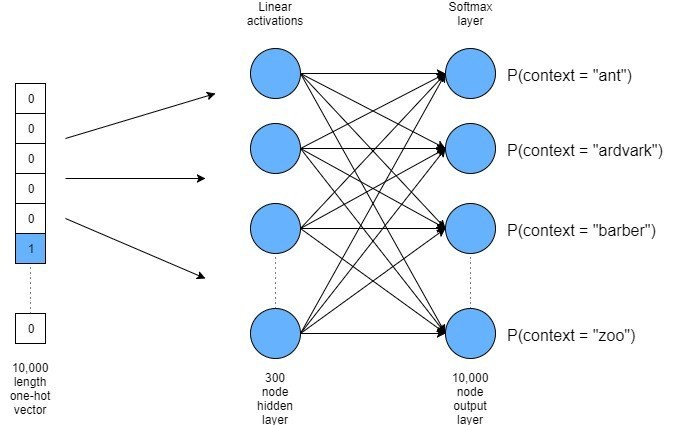
\includegraphics[width=.9\textwidth]{embeddings_example.jpeg}
\end{frame}

\begin{frame}{Embeddings in math}
(a simple) Embedding model:
\[
\bm{D} = s\left(\bm{D\Gamma}_0\bm{\Gamma}_1\right) + \epsilon
\]
where:
\begin{itemize}
\item $\bm{D}$ is the document matrix, dimension $N\times V$
\item $\bm{\Gamma}_0$ is the first weight matrix.  It has dimension $V \times U$, where $U << V$.  It is responsible for ``embedding'' $\bm{D}$ in a lower-dimensional space
\item $\bm{\Gamma}_1$ is the second weight matrix.  Its dimension is $U \times V$.  It is responsible for taking the lower-dimensional representation and bringing it back to the original resolution.
\item $s()$ is the softmax function.  It maps the maps real numbers to a vector of probabilities summing to 1.
\item $\epsilon$ is the error to be minimized.  As the bottleneck gets skinnier (i.e.: as $U$ gets smaller), $\epsilon$ will have to increase.
\end{itemize}
\end{frame}

\begin{frame}{Embeddings in math}
(a simple) Embedding model:
\[
\bm{D} = s\left(\bm{D\Gamma}_0\bm{\Gamma}_1\right) + \epsilon
\]
where:
\begin{itemize}
\item The embedded text, call it $\bm{E}$, is defined as $\bm{D\Gamma_0}$ (dimension $N \times U$)
\item (most) Embedding models are trained by computing the derivatives of the parameter matrices $\bm{\Gamma}_0, \bm{\Gamma}_1$ with respect to a loss function, changing the parameters to make the loss smaller, and then recomputing the derivatives and repeating.  This is backpropagation.
\item the error $\epsilon$ is implicit.  The goal is to minimize it, to get the best possible $\bm{\Gamma}$.  But as the dimension of $\bm{\Gamma}$ gets smaller, this gets harder to do.
\end{itemize}
\end{frame}

\begin{frame}{Embeddings in practice}
Training and using embeddings are separate processes.  Trained embedding models give you $\bm{\Gamma}_0$.  You then supply your own text to multiply it against.  For example, take $\bm{D}$ to be our doctor Seuss example from before.  The embeddings $\bm\Gamma_0$ might look like this:
\[  \bm{\Gamma}_0 \equiv
\begin{array}{c|cccccc}
     & u1 & u2 \\
     \hline
I    & 1 & 2 \\
am   & 3 & 4  \\
Sam  & 5 & 6   \\
would& 7 & 8  \\
you  & 9 & 10  \\
like & 11 & 12  \\
\end{array}\] 
(Note that the entries of the matrix are totally unrealistic in this example)

\end{frame}

\begin{frame}{Embeddings in practice}
Say you wanted to embed the phrase ``I like Sam'' into this two-dimensional space:

\[ 
\left[
\begin{array}{c|cccccc}
I    & 1 & 0  & 0   & 0     & 0   &  0 \\
like & 0 & 0  & 0   & 0     & 0   &  1 \\
Sam  & 0 & 0  & 1   & 0     & 0   &  0 \\
\end{array}\right]
\left[\begin{array}{c|cccccc}
     & u1 & u2 \\
     \hline
I    & 1 & 2 \\
am   & 3 & 4  \\
Sam  & 5 & 6   \\
would& 7 & 8  \\
you  & 9 & 10  \\
like & 11 & 12  \\
\end{array}\right] = 
\left[
\begin{array}{c|cccccc}
     & u1 & u2 \\
     \hline
I    & 1 & 2 \\
like & 11 & 12  \\
Sam  & 5 & 6   \\
\end{array}
\right]
\] 
Because the the document matrix $\bm{D}$ has only one ``1'' per row, this matrix multiplicaton is the same as a ``lookup'' operation.

Still, the matrix notation will come in handy later.

\end{frame}


\begin{frame}{Word embeddings to sentence or span embeddings}
Supervised learning jobs can all be conceptualized as 
\[
y = f(\bm{X}) + \epsilon
\]
where $y$ is some label and $\bm{X}$ is a matrix of features.  So let's add a label to our toy example:


\[
\begin{array}{c|cccccc|c}
     & I & am & Sam & would & you & like & \text{\textbf{label}}\\
     \hline
I    & 1 & 0  & 0   & 0     & 0   &  0  & 0\\
am   & 0 & 1  & 0   & 0     & 0   &  0  & 0\\
Sam  & 0 & 0  & 1   & 0     & 0   &  0  & 1\\
Sam  & 0 & 0  & 1   & 0     & 0   &  0  & 0\\
I    & 1 & 0  & 0   & 0     & 0   &  0  & 0\\
am   & 0 & 1  & 0   & 0     & 0   &  0  & 0\\
would& 0 & 0  & 0   & 1     & 0   &  0  & 1\\
you  & 0 & 0  & 0   & 0     & 1   &  0  & 1\\
like & 0 & 0  & 0   & 0     & 0   &  1  & 0\\
\end{array}\] 
(I labeled words that come after a verb)
\end{frame}

\begin{frame}{Word embeddings to sentence or span embeddings}
If we fit 
\[
\text{\textbf{label}} = f(\bm{D}) + \epsilon
\]
or 
\[
\text{\textbf{label}} = f(\bm{E}) + \epsilon
\]
our model would do nothing but capture the correlations between individual words and labels.  But what if we want to capture the surrounding context?

First, let's remember that the matrix equation above is the same as 
\[
label_i = f(E_i) + \epsilon
\]
where $i$ indexes rows from 1 to $N$.  A natural strategy could be to include lags and leads:
\[
label_i = f(E_i, E_{i-1}, E_{i+1}) + \epsilon
\]
But lots of other possibilities exist.
\end{frame}


\begin{frame}{Word embeddings to sentence or span embeddings}
Consider the span ``I am Sam''.  Its embedding is:
\[\left[\begin{array}{c|cc|c}
     & u1 & u2 & \text{\textbf{label}}\\
     \hline
I    & 1 & 2 & 0\\
am   & 3 & 4 & 0 \\
Sam  & 5 & 6 & 1  \\
\end{array}\right]\]
The centroid word is ``am'', which is associated with a label of zero.  How do we associate information about the surrounding words with that zero label?  Several options, all of which involve ``windowing'':
\begin{itemize}
\item Lags and leads
\item span-wise maxes and mins, averages
\end{itemize}
\[\left[\begin{array}{c|cc|c|cc|cc|cc|cc}
     & u1 & u2 & \text{\textbf{label}} & \multicolumn{2}{c|}{lag}& \multicolumn{2}{c|}{lead} & \multicolumn{2}{c}{min}& \multicolumn{2}{c|}{max}\\
     \hline
am   & 3 & 4 & 0 &1 &2 & 5 & 6 &1 &2 & 5 & 6\\
\end{array}\right]\]

In this toy example, the lags and leads happen to be the same as the maxes and mins, but that won't generally be the case.
\end{frame}

\begin{frame}{Word embeddings to sentence or span embeddings}
We've been working with a bandwidth of 1 (as measured from the centroid.). This is the same thing as a window size of 3.

Taking an average over this window is the same as doing the following:
\[[.33, .33,  .33]\left[\begin{array}{c|cc}
     & u1 & u2\\
     \hline
I    & 1 & 2\\
am   & 3 & 4\\
Sam  & 5 & 6\\
\end{array}\right]
= [3, 4]
\] 
But why weight evenly?  We could do
\[[.2, .7,  .1]\left[\begin{array}{c|cc}
     & u1 & u2\\
     \hline
I    & 1 & 2\\
am   & 3 & 4\\
Sam  & 5 & 6\\
\end{array}\right]
= [2.8, 3.8]
\] 
Optimal weighting schemes could be hyperparameters.  Or they could be \textit{directly estimated} at the same time as model parameters if we're using a neural network.  This is very similar to the concept of \textit{attention}.
\end{frame}

\begin{frame}{Embedded Ngrams}
Ngrams are usually computed over the whole of a document, but they could also be computed over a window.  Here's bigrams for our dummy example:
\[\bm{G}^2 = {\displaystyle
\begin{array}{c|cccccc}
     & (I,I) & (I, am) & (I, sam) & \hdots & (am, Sam) & (Sam, Sam)\\
     \hline
I    & 0 & 1 & 0 & \hdots & 0 & 0\\
am   & 0 & 1 & 0 & \hdots & 1 & 0\\
Sam  & 0 & 0 & 0 & \hdots & 1 & 0\\
\end{array}}
\]
These bigrams are going to be much too high-dimensional to use as-is, but we can embed them into a lower-dimensional space:
\[
E^2 = \underbrace{\bm{G}^2}_{N\times V^2}\left[\underbrace{\bm{\Gamma}_0\otimes \bm{\Gamma}_0}_{V^2 \times U^2}\right]
\]
Doing so could help capture topology-dependent phenomena like negation and adjectives/adverbs.  The dimensionality is too high to do this with the whole vocab even at $U = 100$, but this could be reduced through TF-IDF weighting of bigrams and PCA on the matrix $\bm\Gamma$.
\end{frame}

\begin{frame}{Models}
Given a label and a transformation that takes the document matrix $\bm{D}$ and returns $\bm{X}$, fitting a statistical model is generally a fairly straightforward exercise of tuning hyperparameters.  

Neural nets are the exception, because they effectively create their own design matrices through representation learning.  I'll discuss those later.

We'll try:
\begin{itemize}
\item Penalized logistic regression
\item Random forests
\item XGboost (with trees, probably)
\end{itemize}
\end{frame}

\end{document}